\bigskip
\textit{This paper is the report of the \textbf{Group 43} for the first assignment
of the course.}

\section{Search Algorithms and their relations}

\begin{enumerate}
 \item Give a consistent heuristic for this problem. Prove that it is admissible.
    \begin{framed}
        Our heuristic is a function of the distance with a manhattan
        distance heuristic (ignoring walls) between
        the current character position and the \euro{} position. It is
        admissible because it will never overestimate the cost of reaching
        the goal, as such we will always find an optimal solution with A*
        search. 
    \end{framed}
 \item Show on the left maze the states (board positions) that are visited during an
execution of a uniform-cost graph search. We assume that when different states
in the fringe have the smallest value, the algorithm chooses the state with
the smallest coordinate (\textit{i, j}) ((0, 0) being the bottom left position, \textit{i} being the
horizontal index and \textit{j} the vertical one) using a lexicographical order.
    \begin{framed}
        \begin{center}
        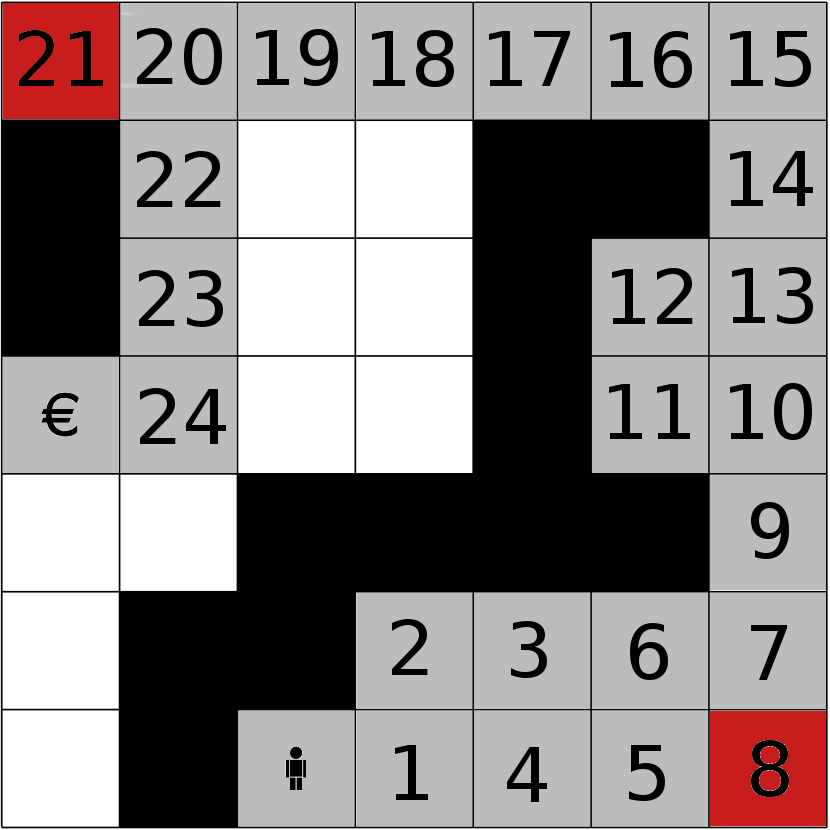
\includegraphics[width=0.5\linewidth]{figure1_left.png}
        \end{center}

        The squares are visited following the numbering order and red nodes
        are not included in the final path. 
    \end{framed}
  \item Show on the right maze the board positions visited by A graph search with
a manhattan distance heuristic (ignoring walls). A state is visited when it is
selected in the fringe and expanded. When several states have the smallest
path cost, this uniform-cost search visits them in the same lexicographical order
as the one used for uniform-cost graph search.
    \begin{framed}
        \begin{center}
        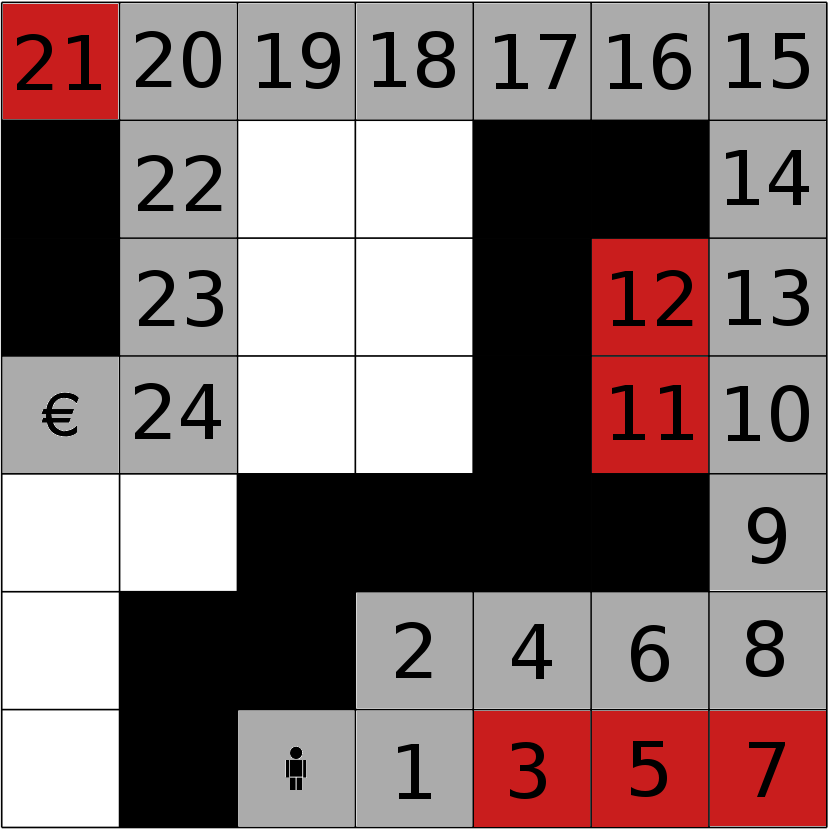
\includegraphics[width=0.5\linewidth]{figure1_right.png}
        \end{center}

        The squares are visited following the numbering order and red nodes
        are not included in the final path. 
    \end{framed}

\end{enumerate}

\section{Sokoban planning problem}

\begin{enumerate}
 \item As illustrated on Figure 3 some situations cannot lead to a solution. Are there
other similar situations? If yes, describe them.
  \begin{framed}
        Other similar situations that cannot lead to a solution happen :
        \begin{itemize}
            \item When a box is in a corner formed by walls and
                this corner is not a target position for boxes ;
            \item When two boxes are next to each other and both of the boxes cannot be moved so they act as
                walls.
        \end{itemize}
  \end{framed}
  \item Why is it important to identify dead states in your successor function? How
are you going to implement it?
    \begin{framed}
        Identifying as many dead states as possible will allow us to reduce
        the search space by stopping the exploration of branches that fell
        in a dead state. Allowing us to reduce the time that our algorithm
        need to find a solution. We are going to implement it by
        identifying the situations mentioned in the answer to the previous
        question.
    \end{framed}
  \item Describe possible (non trivial) heuristic(s) to reach a goal state (with reference
if any). Is(are) your heuristic(s) admissible and/or consistent?
    \begin{framed}
    A first interesting heuristic would be to give a fixed penalty for each
    boxes that isn't on a target, allowing our algorithm to investigate
    potential solution first. But this heuristic that is neither consistent
    nor always admissible (depending on the penalty) has a quite a few
    shortcoming as it might take a long time before the algorithm finds a
    state worth investigating and that, if a box has to reach a target by
    passing over another target, it will explore all the children of this
    state before considering other solution. \newline

    A second interesting heuristic, that solve the shortcomings of the
    previous one, would be the sum of the manhattan distance from each
    boxes to the closest target. Although this heuristic is not always
    consistent as two boxes could calculate the manhattan distance with the
    same target, it is always admissible as it won't ever overestimate the
    cost to reach a solution. As this heuristic is also fast to compute, it
    is extremely interesting to implement it or a close derivative in our
    solution.
    \end{framed}
  \item Implement this problem. Extend the \textit{Problem} class and implement the necessary
methods and other class(es) if necessary. Your file must be named \textit{sokoban.py}.
You program must print to the standard output a solution to the sokoban instance
given in argument satisfying the described format. You will receive the name
of the instance and you have to read from the two files .init and .goal, for
instance, given instance instance1 you will read from files instance1.init
and instance1.goal .
    \begin{framed}
        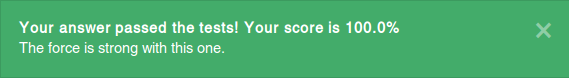
\includegraphics[width=0.8\linewidth]{test_passed.png}
    \end{framed}
  \item Experiment, compare and analyze informed (\textit{astar\_graph\_search}) and unin-
formed (\textit{breadth\_first\_graph\_search}) graph search of aima-python3 on the 15
instances of sokoban provided. Report in a table the time, the number of
explored nodes and the number of steps to reach the solution. Are the
number of
explored nodes always smaller with \textit{astar\_graph\_search}, why?
When no solution can be found by a strategy in a reasonable time (say 5 min),
explain the reason (time-out and/or swap of the memory).
    \begin{framed}
    	\begin{tabular}{l|l|l}
    					& A* 		& Breadth-first\\
            \hline
    		sokoInst01 	& 9ms		& 180ms \\
    					& 71		& 2790 \\
    					& 15		& 15 \\
    		sokoInst02 	& 1s66		& 1s94 \\
    					& 20947 	& 30368 \\
    					& 65		& 65 \\
    		sokoInst07 	& 450ms		& 710ms \\
    					& 5311		& 9394 \\
    					& 98		& 98 \\
    		sokoInst08 	& 600ms		& 940ms \\
    					& 6679		& 13628 \\
    					& 108		& 90 \\
    		sokoInst15 	& 15s		& 68s27 \\
    					& 146013 	& 802991 \\
    					& 68		& 56 \\
    	\end{tabular}

        The number of explored with an A* graph search is always smaller or
        equals to the BFS, smaller if the heuristic is good and put on the
        worst cases a big weight ; equals if the heuristic is very bad.
    \end{framed}
  \item What are the performances of your program when you don’t perform dead state
detection?
    \begin{framed}
      \todo[inline]{Réponse à faire}
    \end{framed}
\end{enumerate}
